\documentclass[dvipdfmx,a4paper,11pt]{jsbook}

\usepackage{amsmath,amsfonts}
\usepackage[mathcal]{euscript}
\usepackage{mathtools}
\usepackage{xcolor}
\usepackage{xcoffins,calc}
\usepackage{bm}
\usepackage{amsthm}
\usepackage{amssymb}
\usepackage{pgf}
\usepackage{titlesec}
\usepackage{ifthen}
\usepackage{mathrsfs}
\usepackage[scr]{rsfso}
\usepackage{relsize}
\usepackage{makeidx}
\usepackage{etoolbox}
\usepackage{footnote}
\usepackage[all]{xy}
\usepackage{url}
\usepackage[most]{tcolorbox}

\usepackage[%
dvipdfmx, %欧文ではコメントアウトする
setpagesize=false,
bookmarks=true,
bookmarksdepth=tocdepth,
bookmarksnumbered=true,
colorlinks=true,
linkcolor=blue,
citecolor=blue,
urlcolor=blue,
pdftitle={},
pdfsubject={},
pdfauthor={},
pdfkeywords={}
]{hyperref}


\tcbset {
  base/.style={
    arc=0mm, 
    bottomtitle=0.5mm,
    boxrule=0mm,
    colbacktitle=black!10!white, 
    coltitle=black, 
    fonttitle=\bfseries, 
    left=2.5mm,
    leftrule=1mm,
    right=3.5mm,
    title={#1},
    toptitle=0.75mm, 
  }
}

\definecolor{brandblue}{rgb}{0.34, 0.7, 1}
\newtcolorbox{mainbox}[1]{
  colframe=brandblue,
  breakable=true, 
  base={#1}
}

\newtcolorbox{subbox}[1]{
  colframe=black!30!white,
  breakable=true,
  base={#1}
}

\usepackage{listings,jvlisting} %日本語のコメントアウトをする場合jvlisting(もしくはjlisting)が必要
%ここからソースコードの表示に関する設定
\lstset{
  basicstyle={\ttfamily},
  identifierstyle={\small},
  commentstyle={\smallitshape},
  keywordstyle={\small\bfseries},
  ndkeywordstyle={\small},
  stringstyle={\small\ttfamily},
  frame={tb},
  breaklines=true,
  columns=[l]{fullflexible},
  numbers=left,
  xrightmargin=0zw,
  xleftmargin=3zw,
  numberstyle={\scriptsize},
  stepnumber=1,
  numbersep=1zw,
  lineskip=-0.5ex
}


\usepackage{pxjahyper}
\usepackage{tikz}
\usetikzlibrary{intersections,calc,arrows.meta,arrows}
\usetikzlibrary{hobby}
\usetikzlibrary{decorations.markings}
\usepackage{wrapfig}
\usepackage[truedimen,top=25truemm,bottom=30truemm,hmargin=25truemm]{geometry}
\usepackage{calc}
\usepackage{fancyhdr}
\pagestyle{fancy}

\begin{document}

\setlength{\footskip}{20truemm}

\makeatletter
\newcount\@chars\newcount\@lines
\@chars=40                      % 1行の文字数
\@lines=40                      % 1ページの行数

\newdimen\@kanjiskip
\@kanjiskip=\dimexpr(\textwidth-1zw*\@chars)/\numexpr\@chars-1
\newdimen\@@kanjiskip
\@@kanjiskip=\dimexpr\@kanjiskip/10

\baselineskip=\dimexpr\textheight/\@lines
\kanjiskip=\@kanjiskip plus \@@kanjiskip minus \@@kanjiskip
\parindent=\dimexpr 1zw+2truept
\parindent=\dimexpr\parindent+\@kanjiskip
\makeatother


\title{Linuxサーバーの導入}
\author{山内優弥}
\date{\today}
\maketitle

\setcounter{tocdepth}{2}
\tableofcontents
\clearpage

\section{この文書について}
Linuxのディストリビューションの一つであるUbuntuの導入からサーバーとしての利用の手順を
述べて文書である.また
\begin{mainbox}{ああああ}
  あああああ
\end{mainbox}
や
\begin{subbox}{いいいい}
  いいいいい
\end{subbox}
で書かれる文章は必ず読む必要はなく適当な補足であることにする.
\section{実行環境} 
\chapter{Ubuntuの導入}
\section{Ubuntuのダウンロード}
今回はUbuntu Japanese Teamから日本語環境のUbuntuのダウンロードをこのページ\url{https://www.ubuntulinux.jp/japanese}
からダウンロードします.どのミラーサイトを用いても構いません.
\begin{mainbox}{Ubuntuの日本語環境のバージョンについて}
  今現在(2024/10/21)最新のLTS(Long-Term Support)バージョンはUbuntu 24.04.1 LTSだが,
  2024/06/10の記事(\url{https://www.ubuntulinux.jp/News/ubuntu2404-ja-remix})において
  Ubuntu Japanese TeamがUbuntu 24.04 LTSの日本語Remixをリリースしないことを表明しています.
\end{mainbox}

\begin{subbox}{Ubuntuの歴史}
  Ubuntuは,2004年にリリースされたLinuxディストリビューションで,Debianをベースにしています.
  開発元はCanonicalという会社で,
  創設者のMark Shuttleworthによって立ち上げられました.Ubuntuの
  名称は南アフリカのズールー語で「他者への思いやり」や「人間性」を意味し,
  オープンソースコミュニティやユーザー間での協力を象徴しています.
  \begin{itemize}
    \item 2004年: 最初のバージョン「Ubuntu 4.10 "Warty Warthog"」がリリースされました.
    Debianベースで使いやすさを重視し,デスクトップLinuxの普及を目指しました.
    \item 2006年: LTS(Long Term Support)リリースが導入され,「Ubuntu 6.06 LTS "Dapper Drake"」が最初のLTS版です.
    LTS版は5年間の長期サポートが提供され,企業や組織での採用が進みました.
    \item 2010年: Ubuntuはデフォルトのデスクトップ環境をGNOMEからUnityに変更しました.Unityはユーザーインターフェースを刷新し,
    使いやすさを向上させることを目的としていましたが,一部のユーザーから批判もありました.
    \item 2017年: Unityの開発が中止され,GNOMEデスクトップに戻ることが発表されました.「Ubuntu 17.10 "Artful Aardvark"」
    でUnityからGNOMEへの移行が行われ,従来のデスクトップ環境を採用する形に戻りました.
    \item 2020年代以降: クラウドやIoT(モノのインターネット),サーバー市場でもUbuntuは広く利用されています.また,
    Ubuntuベースの派生ディストリビューション(Kubuntu,Xubuntu,Lubuntuなど)がそれぞれのニーズに応じて発展してきました.
  \end{itemize}
\end{subbox}

\begin{mainbox}{isoファイルについて}
  気が向いたら書く.
\end{mainbox}


\section{rufus}

rufusとはブータブルUSB作成するソフトウェアで次のURLからダウンロードできる.
\url{https://rufus.ie/ja/#google_vignette}\\
USBを挿してrufusを開くと次のようなウィンドウが出現する.
\begin{figure}[htbp]
  \begin{center}
    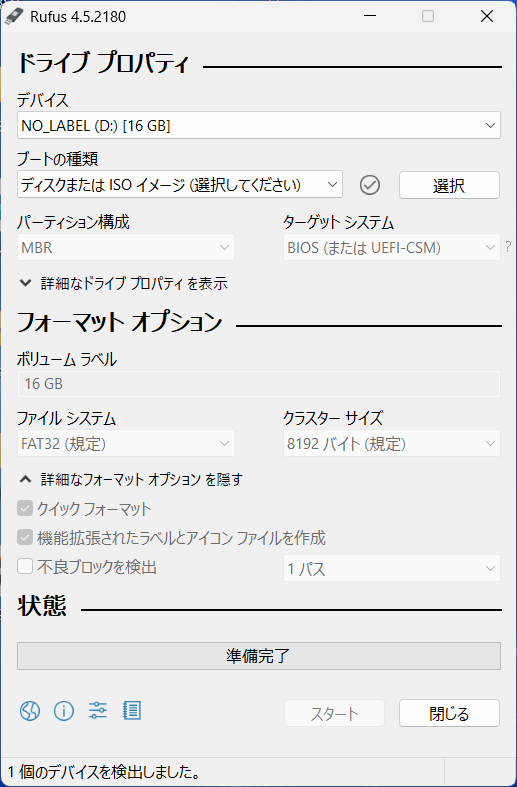
\includegraphics[width = 50mm]{rufus.png}
    \caption{rufusのウィンドウ}
  \end{center}
\end{figure}
\\
「選択」から先程ダウンロードしたUbuntuのisoファイルを選択して,スタートを選択する.これでUbuntuを起動する準備が整った.

\section{Ubuntuとの邂逅}
BIOSを起動して,Bootの順位を変更してUbuntuを一番上に変更する.
これによりUbuntuが起動する.





\end{document}
